\documentclass[a4paper,12pt]{UoBnote}

\usepackage{enumitem}
\usepackage{listings}
\usepackage{color}
\usepackage{graphicx}
\usepackage{amsfonts}
\usepackage[backend=bibtex]{biblatex}

\addbibresource{bilbo.bib}

\lstset{language=sh}
\setlength{\parskip}{1em}
\author{Mike Knee}

\shorttitle{Numerical Modelling}
\title{Worksheet 1 Report}
\date{\today}
\issue{1}

\begin{document}

\maketitle
\tableofcontents
\vspace{1cm}\hrule \vspace{1cm}

\section{Question 1}

For the first excercise a number of commands were input to the linux bash prompt, in order to understand what the different commands do and how to use them. The commands are listed here in order, with the output following and finally a description of what the command has done.
\begin{enumerate}[label=\alph*)]
	\item mkdir compphys

		No output, but a new directory has been created called ``compphys''
	\item cd compphys

		No output again, but now the current working directory is ``~/compphys''
	\item cat $>$ file1.txt [rtn] this is my first file [rtn][ctrl-c]

		No output is printed to the screen, however a new file called ``file1.txt'' has been created, containing the text ``this is my first file''
	\item ls

		Ouput is: 
		\begin{verbatim}
		file1.txt
		\end{verbatim}

		The ls command lists the contents of the current working directory.
	\item more file1.txt

		Output is:
		\begin{verbatim}
		this is my first file
		\end{verbatim}

		The more command pages files to the standard output, seen as the file ``file1.txt'' only has one line, that line is simply printed to the terminal.
	\item xclock\&

		Output is shown in figure \ref{fig:xclock}.
		\begin{figure}
			\centering
			
\includegraphics{xclock}
			\caption{xclock open through the ssh session}
			\label{fig:xclock}
		\end{figure}

		The xclock\& command starts an xclock process. This will be opened on the client side through ssh if X11 forwarding is enabled, and the client is able to display xwindow objects. The ampersand is to tell the process to start the process in the background, ie. to allow the shell session to continue while xclock is still running.
	\item whoami

		Output is:
		\begin{verbatim}
		mfk364
		\end{verbatim}

		This command prints the username of the current user.

	\item man ls

		Output is a man page, a text document describing the usage of the ``ls'' command. Calling man $<$command$>$ will display a man page on any command with proper documentation. Figure \ref{fig:manpage} shows the top of the ls man page.
		\begin{figure}
			\centering
			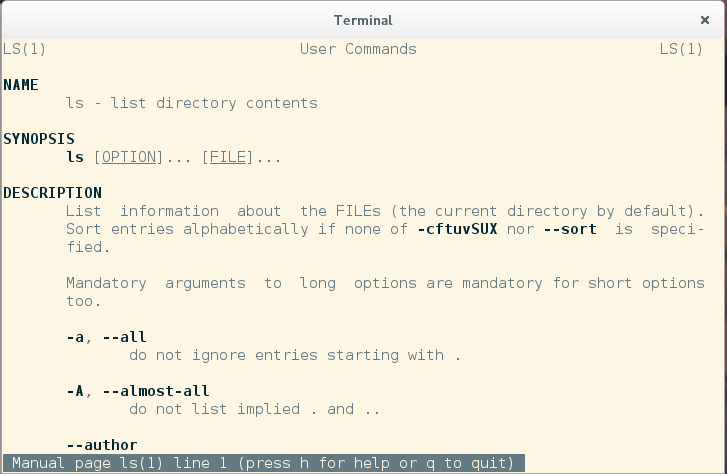
\includegraphics[scale=0.5]{manls}
			\caption{Top of the man page for the ``ls'' command}
			\label{fig:manpage}
		\end{figure}

	\item top

		Output is a display of running processes, ordered by CPU usage. The column processes are sorted by, and other options can be changed using commands while top is running. Figure \ref{fig:top} shows top while running, with the columns sorted by CPU usage.
		\begin{figure}
			\centering
			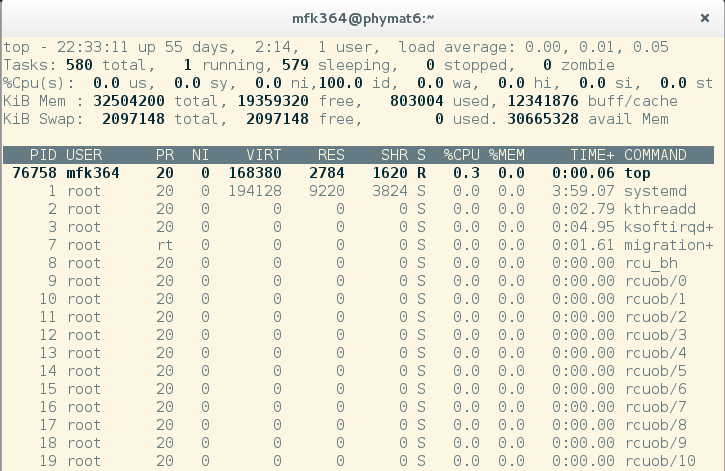
\includegraphics[scale=0.5]{top}
			\caption{The ``top'' command in action}
			\label{fig:top}
		\end{figure}

	\item kill

		The ``kill'' command is used to stop running processes. In order to use kill one needs the PID of the process to be stopped. For this the ``ps'' command is used, which lists all the processes running under the current user's UID. Once a PID is known ``kill [PID]'' will send a terminate signal to the process.

		The output of the kill command is:
		\begin{verbatim}
		[running processes] Terminated\tab [process name]
		\end{verbatim}

	\item ps -u [username]

		As described above the ``ps'' command displays currently running processes. The -u option denotes that all the processes belonging to a user specified by [username] should be displayed. The default behaviour of ``ps'' is to display the processes belonging to the current user running in the current TTY. 

		An example output of the ``ps -u [username]'' is shown in figure \ref{fig:ps}. 
		\begin{figure}
			\centering
			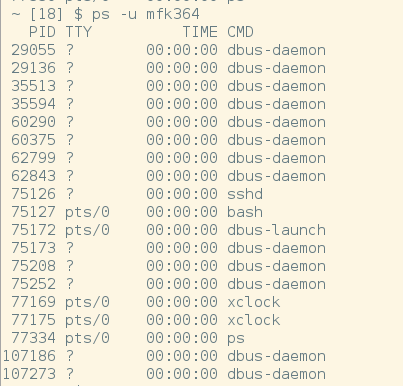
\includegraphics[scale=0.4]{ps}
			\caption{An example of ``ps -u [username]'' output}
			\label{fig:ps}
		\end{figure}

\end{enumerate}

\section{Question 4}


For this question a C++ program was required to calculate different powers of $\phi$ (the silver ratio), given by $\phi = \frac{-1 + \sqrt{5}}{2}$, and output the data to a file. The source code for this program is called ``w1q4.cpp'', and when run will output data to a file called ``output''. The code calculates and writes the power of phi by basic multiplication in lines 53-56.

The recursion relation \[\phi^{n+1}=\phi^{n-1}-\phi^{n}\] can be shown by noting that if we multiply both sides by $\phi$ we get \[\phi^{n+2}=\phi^{n}-\phi^{n+1}\] we can then substitute $m=n+1$ to give us \[\phi^{m+1}=\phi^{m-1}-\phi^{m}\] This means the recursion relation is always valid for any value of $n\in\mathbb{Z}, n\geq n_0$ as long as the base case $n_0$ is defined for $n$ (as we can see $m$ must also be an integer greater than $n_0$).

The base case is relatively easy to show using the properties of the golden ratio, and by extension its conjugate which we are interested in. It is easiest to show by taking the case that $n_0=0$, especially when we note that a property of the golden ratio (see reference \cite{goldenratio}) ($\Phi$) is \[\frac{1}{\Phi}=\Phi-1\] and therefore, because the silver ratio $\phi=\frac{1}{\Phi}$, that the silver ratio has a similar property \[\frac{1}{\phi}=\phi+1\] If we now take our recursion relation with $n=0$ \[\phi^1=\phi^{-1}-\phi^0\] \[\phi=\frac{1}{\phi}-1\] we can see that the recursion relation is satisfied by considering the properties of the silver ratio as the conjugate of the golden ratio.

The function \texttt{recursion\_relation} (starting at line $20$ in the code) is the reursive function that uses the recursion relation defined as $\phi^{n+1}=\phi^{n-1}-\phi^{n}$. When the programme is run with values of $N$ greater than around $40$ the programme runs extremely slowly. This is because this recursive function runs in $O(n^2)$ time, and is therefore very slow.

We can see by looking at the results that the two recursive functions both fail with varying degrees of severity. The function using floats begins to fluctuate relatively quickly, and produces very poor results. The double precision recursive function performs better, however it still produces fluctuations and innacuracies compared to our reference value calculated using direct multiplication.

\section{Question 6}

In this problem we consider a mass suspended by two springs from a bench, as shown in figure \ref{fig:masses}. We need to find the angle $\theta$ that the two spings make with the bench in terms of the known quantities: the length of the bench $L$, the mass $m$, and the spring constant $k$. The springs both have natural length $L/2$.

The equation for $theta$ can be found by balancing forces. If we start with the equation \[mg=2T\sin{\theta}\] where $T$ is the tension in one spring, we can use the equation \[T=k\Delta x\] We then find $\Delta x$ in terms of the $L$ and $\theta$ \[\Delta x=\frac{L}{2\cos{\theta}}-\frac{L}{2}\] \[T=k\frac{L}{2}(\frac{1}{\cos{\theta}}-1)\] If we now substitute back into our first equation then we get \[mg=kL(\tan{\theta}-\sin{\theta})\]

We will use values $m=5.5$kg, $L=0.6$m and $k=850$N. The code uses a recursive function to calculate and output the result using the bisection method of root finding (see chapter 03.03 in reference \cite{holistic}). A precision of 6 significant figures is used, with our initial ``bracket'' around the root being $0$ and $\pi/2$. By considering the physical properties of the system it is clear that these are sensible choices for out initial lower and upper bounds as $\theta$ must lie between these two points. The error at each iteration is given by half the difference between the upper and lower bounds, as we know the root must lie somewhere between this boundary and therefore cannot be more than half the difference from the centre of the boundary. Once the difference between the upper and lower bounds is less than our required precision we take the average of the upper and lower bound, and this gives us our answer to our chosen significant figures. 

\begin{figure}
	\centering
	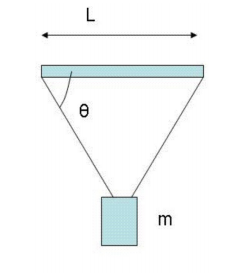
\includegraphics[scale=1]{masses}
	\caption{Mass suspended from a bench by two springs.}
	\label{fig:masses}
\end{figure}

\section{Question 7}

Here we are considering the error propogation when using the bisection and Newton-Raphson methods for root finding. We can analyse the error when using the bisection method by considering that if at step $n$ we have upper and lower bound $u_n$ and $l_n$, middle value $m_n=\frac{u_n+l_n}{2}$ and error $\epsilon_n=\frac{u_n-l_n}{2}$. We can then say that our new boundaries will be one of $u_n$ or $l_n$ along with $m_n$, which has error $epsilon_n$ associated with it. If we assume that the error in the value of $u_n$/$l_n$ is negligible compared to $epsilon_n$ then we can see that the middle on the $n+1$ iteration is \[m_{n+1}=\frac{|m_n+\epsilon_n-(u_n\, or\, l_n)|}{2}\] This shows us simply that the error is halved on each iteration, giving us: \[\epsilon_{n+1}=\frac{\epsilon_n}{2}\]

Next let us consider the error given at each iteration by the Newton-Raphson method. If we perform a taylor expansion of the function about the root $x_{root}$ with the value $x=x_n$ we get
\[f(x_n)=f(x_{root}+f'(x_{root})(x_n-x_{root})+\frac{1}{2}f''(x_{root})(x_n-x_{root})^2+...\]
If we then note that the absolute error at each iteration is given by the difference between the value at each iteration and the actual root
\[\epsilon_n=x_n-x_{root}\]
and substitute this into our taylor expansion above (and also noting that $f(x_{root})=0$) we get
\[f(x_n)=f'(x_{root})\epsilon_n+\frac{1}{2}f''(x_{root})\epsilon^2\]
We can define the error at the $n+1$ step as the error at the $n$ step plus the difference in the values at each step, i.e.
\[\epsilon_{n+1}=\epsilon_n+x_{n+1}-x_n\]
From the Newton-Raphson algorithm we can see that
\[x_{n+1}-x_n=frac{f(x_n)}{f'(x_n)}\]
and if we substitue this into our error relationship above we get
\[\epsilon_{n+1}=\epsilon_n+\frac{f(x_n)}{f'(x_n)}\]
We can then substitute in the taylor expansion above, and its derivative which is given by
\[f'(x_n)=f'(x_{root})+f''(x_{root})\epsilon_n+...\]
as $epsilon_n$ is linearly related to $x_n$. This then gives us
\[\epsilon_{n+1}=\epsilon_n+\frac{f(f'(x_{root})\epsilon_n+\frac{1}{2}f''(x_{root})\epsilon_{n}^2...}{f'(f'(x_{root})+f''(x_{root})\epsilon_n+...\}\approx\epsilon_n+\frac{f(f'(x_{root})\epsilon_n+\frac{1}{2}f''(x_{root})\epsilon_{n}^2}{f'(f'(x_{root})+f''(x_{root})\epsilon_n}\]
Next we can simply rearrange this equation, to give us
\[\epsilon_{n+1}= \frac{f'(x_{root})\epsilon_n+f''(x_{root})\epsilon_{n}^2-(f'(x_{root})\epsilon_n+\frac{1}{2}f''(x_{root})\epsilon_{n}^2}{f'(f'(x_{root})+f''(x_{root})\epsilon_n}\]
\[\epsilon_{n+1}=\frac{f''(x_{root})\epsilon_{n}^2}{2f'(x_{root})}\]
So we can see that the error at each iteration should decrease quadratically, a large improvement on the bisection method. This relationship above assumes that $f'(x_{root})\neq0$, and if the derivative is 0 then the algorithm will not converge on a root. For further details see reference \cite{newtonsmethod}.

It is possible for the Newton-Raphson method to not converge for other reasons as well. If the chosen initial value for $x_0$ is too close to a local maxima or minima, or too close to an asymptote the method may fail to converge on a root of the equation.

Figure \ref{fig:errorgraph} shows the absolute error over the iterations for three different runs, first using the bisection method and then two seperate runs of the Newton-Raphson method starting from different points. The bisection method starts with upper and lower bound $10$ and $-10$ respectively. The first Newton-Raphson run starts with initial guess $n_0=10$, and the second starts with $n_0=-10$. We can see from the graph that both the Newton-Raphson method runs converge on the root much quicker than the bisection method, which is as we expect as we have already seen that the Newton-Raphson method converges quadratically compared to the bisection methods linear convergance. 

We can also see that the second Newton-Raphson run converges very quickly, within five iterations, which is to be expected as the initial guess input to the algorithm is quite close to the actual root. The first run for the method takes a little bit longer, and has some fluctuations in the error as we converge. 

\begin{figure}
	\centering
	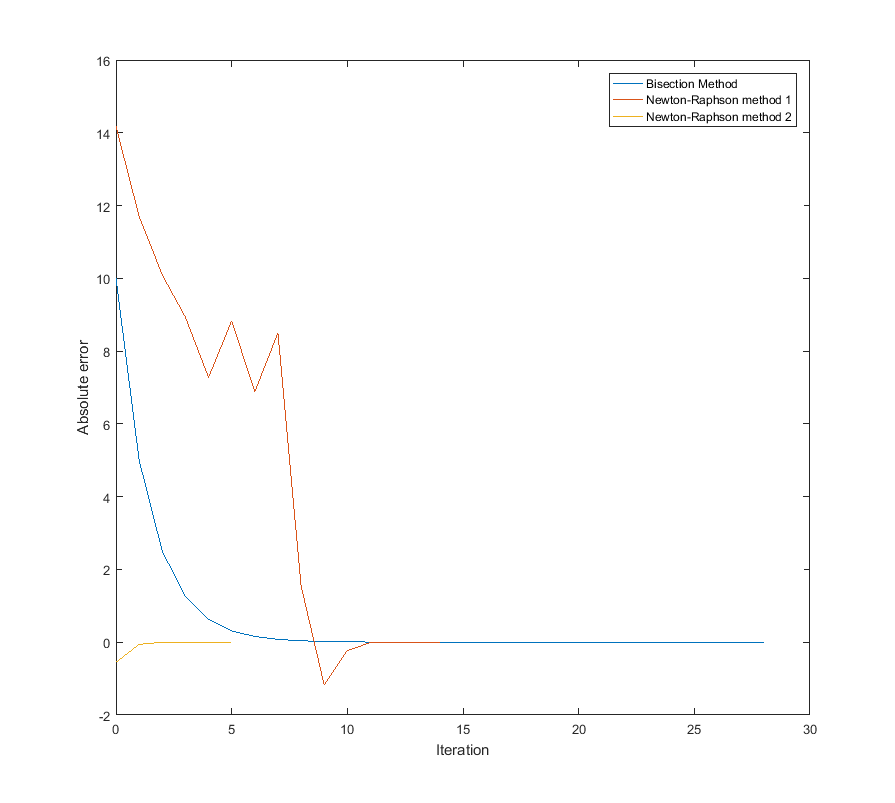
\includegraphics[scale=1]{errorgraph}
	\caption{Graph showing the error at each iteration for the bisection method and two seperate runs of the Newton-Raphson method.}
	\label{fig:errorgraph}
\end{figure}

\printbibliography

\end{document}

